\documentclass[]{beamer}
\usetheme{Boadilla}
\usecolortheme{beaver}
\usepackage[utf8]{inputenc}
\usepackage[american]{babel}
\usepackage[T1]{fontenc}
\usepackage{color}

\newcommand{\semitransp}[2][35]{{\color{fg!#1}#2}}
\newcommand{\ttt}[1]{\texttt{#1}}
\newcommand{\Na}{\mathbb{N}}
\newcommand{\R}{\mathbb{R}}

% Requests the 'color' package
\newcommand{\code}[1]{\colorbox[gray]{0.8}{\texttt{#1}}}

\definecolor{darkgreen}{rgb}{0,0.5,0}
\definecolor{navy blue}{RGB}{0, 0, 99}
\definecolor{rock blue}{RGB}{156, 170, 198}
\definecolor{refs}{gray}{0.7}

\setbeamercolor{attention box}{use={title in head/foot},%
  fg=navy blue, %
  bg=title in head/foot.bg
}

\author[Sobral]{Francisco N. C. Sobral\\ Universidade Estadual de Maringá}

\date[XXIX SEMAT]{XXIX Semana da Matemática\\UEM, 2018}

\title[Mat. Mult.]{Multiplicando matrizes no computador}

% Remove shadows in blocks
\setbeamertemplate{blocks}[rounded][shadow=false]

% Coisas invisiveis ficam meio transparentes
\setbeamercovered{transparent=40} 

% Desabilita os menuzinhos chatos
\setbeamertemplate{navigation symbols}{} 

% Faz com que as tabelas e figuras sejam numeradas
%\setbeamertemplate{caption}[numbered]

% Lists
% Set circles, triangles and change colors
\setbeamertemplate{itemize items}[triangle]
\setbeamertemplate{enumerate items}[circle]
\setbeamertemplate{section in toc}[circle]
\setbeamertemplate{subsection in toc}
{
  \leavevmode
  \leftskip=2em
  {\usebeamercolor[bg]{item projected}$\bullet$}
  \hskip0.5em\inserttocsubsection\par
}

\setbeamercolor{item projected}{ %
  fg=rock blue, %
  bg=navy blue %
}

\setbeamercolor{item}{ %
  fg=navy blue %
}



\begin{document}

\begin{frame}[plain]
\titlepage
\end{frame}

\begin{frame}{Por que reinventar a roda?}

  \begin{itemize}
  \item Entender o funcionamento da linguagem

  \item Entender o funcionamento da memória

  \item Adquirir conhecimento mais profundo de programação

  \item Em Julia: \code{A * B} e \code{A * v} calculam
    eficientemente os produtos matriz-matriz e matriz-vetor
  \end{itemize}

\end{frame}

\begin{frame}{Tópicos}
\tableofcontents
\end{frame}

\section{Notação}

\begin{frame}{Notação}
  
  \begin{onlyenv}<1>
    \begin{itemize}
    \item Vetor
      \[
      v \in \R^n \Rightarrow v =
      \begin{bmatrix}
        v_1\\ \vdots \\ v_n
      \end{bmatrix}
      \]

    \item Vetor transposto
      \[
      v^T =
      \begin{bmatrix}
        v_1 & \cdots & v_n
      \end{bmatrix}
      \]

    \item Produto escalar de vetores $x$ e $y$
      \[
      x^T y =
      \begin{bmatrix}
        x_1 & \cdots & x_n
      \end{bmatrix}
      \begin{bmatrix}
        y_1\\ \vdots\\ y_n
      \end{bmatrix}
      = \sum \limits_{i = 1}^n x_i y_i
      \]
    \end{itemize}
  \end{onlyenv}

  \begin{onlyenv}<2-4>
    \begin{itemize}
    \item Matriz
      \[
      A \in \R^{m \times p} \Rightarrow A =
      \begin{bmatrix}
        a_{11} & \cdots & a_{1p}\\
        a_{21} & \cdots & a_{2p}\\
        & \vdots & \\
        a_{m1} & \cdots & a_{mp}
      \end{bmatrix}
      =
      \alert<3>{
        \begin{bmatrix}
          & A_1 & \\
          & A_2 & \\
          & \vdots & \\
          & A_m &
        \end{bmatrix} 
      }
      =
      \alert<4>{
        \begin{bmatrix}
          & & \\
          A^1 & \cdots & A^p \\
          &  &
        \end{bmatrix}
      }      
      \]
    \item $\alert<3>{i}$-ésima linha de $A$
      \[
      A_{\alert<3>{i}} =
      \begin{bmatrix}
        a_{i1} & \cdots & a_{ip}
      \end{bmatrix}
      \]
    \item $\alert<4>{j}$-ésima coluna de $A$
      \[
      A^{\alert<4>{j}} =
      \begin{bmatrix}
        a_{1j}\\ \vdots\\ a_{mj}
      \end{bmatrix}
      \]
    \end{itemize}
  \end{onlyenv}

\end{frame}

\section{Vetores, matrizes e memória em Julia}

\begin{frame}{Abrindo o \textit{notebook}}

  \begin{center}
    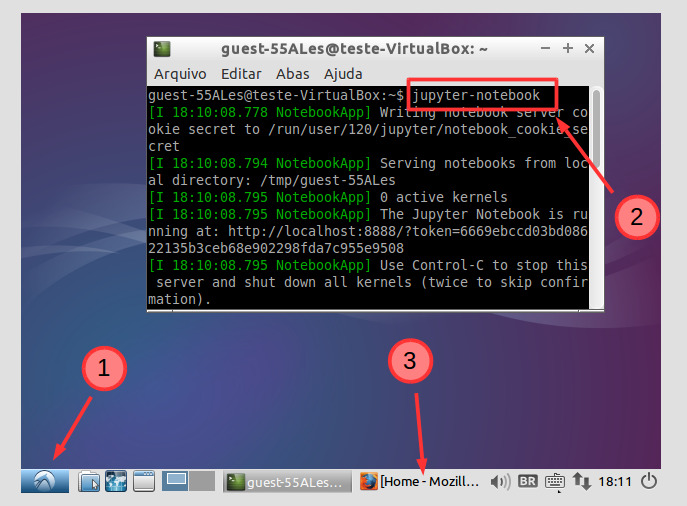
\includegraphics[width=0.85\textwidth]{figures/notebook.png}
  \end{center}

\end{frame}

\begin{frame}[fragile]{Vetores}

  \begin{itemize}
  \item Comando \code{Vector\{Float64\}(n)}

  \item Reserva um espaço na memória de tamanho
    $n \cdot$\verb+sizeof(Float64)+ e retorna o seu \textbf{endereço}

  \item Checamos o endereço com \code{pointer}

  \item[]

  \item \code{zeros(n)}: vetor de zeros
  \item \code{ones(n)}: vetor de uns
  \item \code{rand(n)}: vetor aleatório com números entre 0 e 1

  \item[]

  \item $i$-ésima posição de um vetor $v$: \code{v[i]}
    
    \begin{itemize}
    \item \code{v[2] = 10}: atribuição
    \item \code{v[2] + 10}: conteúdo
    \end{itemize}

  \end{itemize}
  
\end{frame}

\begin{frame}[fragile]{Matrizes}
  
  \begin{itemize}
  \item Comando \code{Array\{Float64\}(m, n)}

  \item Reserva um espaço na memória de tamanho
    $mn\cdot$\verb+sizeof(Float64)+ e retorna o seu \textbf{endereço}

  \item Checamos o endereço com \code{pointer}

  \item[]

  \item \code{zeros(m, n)}: matriz de zeros
  \item \code{ones(m, n)}: matriz de uns
  \item \code{rand(m, n)}: matriz aleatória com números entre 0 e 1

  \item[]

  \item Elemento $(i, j)$ da matriz $M$: \code{M[i, j]}
    
    \begin{itemize}
    \item \code{M[3, 2] = 10}: atribuição
    \item \code{M[3, 2] + 10}: conteúdo
    \end{itemize}

  \end{itemize}
  
\end{frame}

\begin{frame}[fragile]{Percorrendo vetores e matrizes}
  
  \begin{itemize}
  \item Utilizamos laços do tipo \code{for} para percorrer um vetor

    \begin{center}
      \begin{minipage}[c]{0.5\linewidth}
\begin{verbatim}
s = 0.0
for i = 1:n
    s = s + v[i]
end
\end{verbatim}
      \end{minipage}
    \end{center}
    
  \item Para percorrer uma matriz por inteiro, precisamos de
    \alert{dois laços}

    \begin{center}
      \begin{minipage}[c]{0.5\linewidth}
\begin{verbatim}
s = 0.0
for j = 1:n
    # Aqui dentro o j está fixo
    for i = 1:m
        # Aqui dentro o i está fixo
        # j também
        s = s + M[i, j]
    end
end
\end{verbatim}
      \end{minipage}
    \end{center}

  \end{itemize}

\end{frame}

\begin{frame}{Memória}

  \begin{onlyenv}<1>
    \begin{itemize}
    \item Ao criarmos um vetor, um espaço da memória do computador é
      reservado
    \item Quando o vetor não é mais usado, o GC (\textit{Garbage
        Colector}) entra em ação
    \item Criação $>$ Destruição pelo GC $\Rightarrow$ Travamento
    \item Ordem de velocidade de acesso
      \begin{center}
        HD $<$ Memória RAM $<$ \emph{Cache} do processador
      \end{center}
    \item Ordem de espaço disponível
      \begin{center}
        HD (TB) $>$ Memória RAM (GB) $>$ \emph{Cache} do processador
        (MB)
      \end{center}
    \end{itemize}
  \end{onlyenv}

  \begin{onlyenv}<2>
    \begin{itemize}
    \item Matriz $1000\times 1000$ do tipo \code{Float64} ocupa
      \[
      \frac{1000 \times 1000 \times 8}{1024} \approx 8\text{MB}
      \]

    \item Matriz $10000 \times 10000$: 800MB

    \end{itemize}
  \end{onlyenv}

\end{frame}

\begin{frame}{Acessando posições próximas}

  Ao acessar a posição $i$ de um vetor ou $(i, j)$ de uma matriz o
  processador também acessa posições \textcolor{darkgreen}{vizinhas}
  com maior velocidade!

  \begin{itemize}
  \item Uso do \emph{cache}

  \item Se acessou \code{v[5]}, então \code{v[4]} e \code{v[6]} são
    acessadas mais rapidamente que \code{v[20]}

  \item Se acessou \code{M[3, 3]}, então \code{M[2, 3]} e \code{M[4,
      3]} são acessados mais rapidamente que \code{M[3, 4]}

    \[
    \begin{bmatrix}
      1 & 2 & 3 \\
      4 & 5 & 6 \\
      7 & 8 & 9
    \end{bmatrix}
    \quad \Rightarrow \quad
    \begin{bmatrix}
      1 & 4 & 7 & 2 & 5 & 9 & 3 & 6 & 9
    \end{bmatrix}
    \]

  \item Julia é \alert{Orientada a colunas}
  \end{itemize}
  
\end{frame}


\section{Multiplicação de matrizes e vetores}

\begin{frame}{Duas interpretações}
  
  \begin{onlyenv}<1-2>
    Sejam $A \in \R^{m \times n}$ e $v \in \R^n$. Existem duas formas
    de interpretarmos $u = A v$:

    \begin{itemize}
    \item Produto escalar com as \textbf{linhas} de $A$:
      \[
      u =
      \begin{bmatrix}
        \alert<1>{a_{11} v_1} + \cdots + \alert<1>{a_{1n} v_n}\\
        a_{21} v_1 + \cdots + a_{2n} v_n\\
        \vdots \\
        a_{m1} v_1 + \cdots + a_{mn} v_n
      \end{bmatrix}
      =
      \begin{bmatrix}
        \alert<1>{A_1 \cdot v} \\
        \vdots \\
        A_m \cdot v
      \end{bmatrix}
      \]

    \item Combinação linear das \textbf{colunas} de $A$:
      \[
      u =
      \begin{bmatrix}
        \alert<2>{a_{11} v_1} + \cdots + a_{1n} v_n\\
        \alert<2>{a_{21} v_1} + \cdots + a_{2n} v_n\\
        \vdots \\
        \alert<2>{a_{m1} v_1} + \cdots + a_{mn} v_n
      \end{bmatrix}
      = \alert<2>{A^1 v_1} + \cdots + A^n v_n
      \]
    \end{itemize}
  \end{onlyenv}

  \begin{onlyenv}<3>

    \begin{itemize}
    \item Produto escalar
      \[
      u_i = a_{i1} v_1 + \cdots + a_{in} v_n
      \]
      Os elementos de $A$ não estão próximos uns dos outros!

    \item Combinação linear
      \[
      \begin{aligned}
        u_1 & = u_1 + a_{1j} v_j\\
        & \vdots \\
        u_m &  = u_m + a_{mj} v_j
      \end{aligned}
      \]
      Os elementos de $A$ estão próximos uns dos outros!
    \end{itemize}
    
  \end{onlyenv}

\end{frame}

\section{Multiplicação de matrizes}

\begin{frame}{Três interpretações}

  Sejam $A \in \R^{m \times p}$ e $B \in \R^{p \times n}$. Existem
  três formas de interpretarmos $C = A \cdot B$:

  \begin{itemize}
  \item<only@1> Produto escalar
    \[
    \begin{split}
      C & =
      \begin{bmatrix}
        \alert<1>{a_{11} b_{11} + \cdots + a_{1p} b_{p1}} & \cdots &
        a_{11} b_{1n} + \cdots + a_{1p} b_{pn}\\
        & \vdots & \\
        a_{m1} b_{11} + \cdots + a_{mp} b_{p1} & \cdots & a_{m1}
        b_{1n} + \cdots + a_{mp} b_{pn}
      \end{bmatrix} \\
      & =
      \begin{bmatrix}
        \alert<1>{A_1 B^1} & \cdots & A_1 B^n \\
        & \vdots & \\
        A_m B^1 & \cdots & A_m B^n
      \end{bmatrix}
    \end{split}
    \]

    \item<only@2-3> Combinação linear de linhas ou colunas
    \[
    \begin{split}
      C & =
      \begin{bmatrix}
        \alert<2-3>{a_{11} b_{11} + \cdots + a_{1p} b_{p1}} & \alert<2>{\cdots} &
        \alert<2>{a_{11} b_{1n} + \cdots + a_{1p} b_{pn}}\\
        & \alert<3>{\vdots} & \\
        \alert<3>{a_{m1} b_{11} + \cdots + a_{mp} b_{p1}} & \cdots & a_{m1}
        b_{1n} + \cdots + a_{mp} b_{pn}
      \end{bmatrix} \\
      & =
      \begin{bmatrix}
        \alert<2>{A_1 B} \\
        \vdots \\
        A_m B
      \end{bmatrix}
      =
      \begin{bmatrix}
        \alert<3>{A B^1} & \cdots & A B^n \\
      \end{bmatrix}
    \end{split}
    \]

  \item<only@4> Soma de matrizes de posto 1 (\textit{outer product})
    \[
    \begin{split}
      C & =
      \begin{bmatrix}
        \alert<4>{a_{11} b_{11}} + \cdots + a_{1p} b_{p1} & \cdots &
        \alert<4>{a_{11} b_{1n}} + \cdots + a_{1p} b_{pn}\\
        & \vdots & \\
        \alert<4>{a_{m1} b_{11}} + \cdots + a_{mp} b_{p1} & \cdots &
        \alert<4>{a_{m1} b_{1n}} + \cdots + a_{mp} b_{pn}
      \end{bmatrix} \\
      & =
      \alert<4>{
        \begin{bmatrix}
          a_{11} b_{11} & \cdots & a_{11} b_{1n} \\
          & \vdots & \\
          a_{m1} b_{11} & \cdots & a_{m1} b_{1n}
        \end{bmatrix}
      } + \cdots + 
      \begin{bmatrix}
        a_{1p} b_{1p} & \cdots & a_{1p} b_{pn} \\
        & \vdots & \\
        a_{mp} b_{1p} & \cdots & a_{mp} b_{pn}
      \end{bmatrix}
      \\
      & = \alert<4>{A^1 B_1} + \cdots + A^p B_p
    \end{split}
    \]

  \end{itemize}
  
\end{frame}

\section{Problema prático: matrizes esparsas}

\begin{frame}{Matrizes diagonais}

  Seja $D \in \R^{n \times n}$ uma matriz diagonal
  \[
  D =
  \begin{bmatrix}
    d_{11} & 0 & 0 & \cdots & 0 \\
    0 & d_{22} & 0 & \cdots & 0 \\
      & & \ddots & & \\
      & & & \ddots & \\
    0 & 0 & 0 & \cdots & d_{nn}
  \end{bmatrix}
  \]

  \begin{itemize}
  \item $D$ pode ser armazenada no computador em um vetor
    \[
    d =
    \begin{bmatrix}
      d_{11} & d_{22} & \cdots & d_{nn}
    \end{bmatrix}
    \]

  \item Economizamos $n^2 - n$ posições na memória!
  \end{itemize}
  
\end{frame}

\begin{frame}{Multiplicação}
  
  \begin{itemize}
  \item $D \in \R^{n \times n}$ diagonal e $v \in \R^n$
    \[
    D v =
    \begin{bmatrix}
      d_{11} v_1 \\
      \vdots \\
      d_{nn} v_n
    \end{bmatrix}
    \]

  \item $D \in \R^{n \times n}$ diagonal e $A \in \R^{n \times n}$
    qualquer
    \[
    D \cdot A =
    \begin{bmatrix}
      d_{11} a_{11} & \cdots & d_{11} a_{1n} \\
      d_{22} a_{21} & \cdots & d_{22} a_{2n} \\
      & \vdots & \\
      d_{nn} a_{n1} & \cdots & d_{nn} a_{nn} \\      
    \end{bmatrix}
    \]
  \end{itemize}

\end{frame}

\begin{frame}{Matriz esparsa qualquer}

  \begin{onlyenv}<1>
    Considere a matriz
    \[
    A =
    \begin{bmatrix}
      4 & 0 & 2 & 0 & 0 \\
      0 & 5 & 0 & 0 & 0 \\
      0 & 0 & 0 & 0 & 0 \\
      0 & 0 & 0 & 0 & 0 \\
      0 & 0 & 0 & 0 & 0 \\
    \end{bmatrix}
    \]
  
    Como $A$ tem muitos zeros, podemos armazená-la de uma forma
    inteligente através de 3 vetores:

    \begin{itemize}
    \item \code{vi[k]} guarda a linha do $k$-ésimo elemento não nulo
    \item \code{vj[k]} guarda a coluna do $k$-ésimo elemento não nulo
    \item \code{v[k]} guarda o valor do $k$-ésimo elemento não nulo
    \end{itemize}

    \[
    \begin{aligned}
      \text{\code{vi}} & = [1, 2, 1] \\
      \text{\code{vj}} & = [1, 2, 3] \\
      \text{\code{v}} & = [4, 5, 2]
    \end{aligned}
    \]
  \end{onlyenv}

  \begin{onlyenv}<2>
    
    No caso de $A \in \R^{m \times n}$ geral, temos que, se
    \code{vi[k]} $= i$, \code{vj[k]} $= j$ e \code{v[k]} $= x$, então
    \[
    a_{ij} = x
    \]

    \code{length(v)} indica quantos elementos não nulos há em $A$.
    \vfill
    \begin{center}
      \large \alert{Como implementar os produtos?}
    \end{center}

  \end{onlyenv}

\end{frame}

\begin{frame}[plain, noframenumbering]
  \vfill
  \vfill
  \vfill
  \begin{center}
    \Huge Obrigado!
  \end{center}
  \vfill
  \vfill
  \begin{center} \url{fncsobral@uem.br} \end{center}

  \begin{center}
    \href{http://creativecommons.org/licenses/by/4.0/}{
\includegraphics{figures/by.png}} \end{center}
\end{frame}
\end{document}
